\documentclass[11pt]{article}
\usepackage[margin=1in]{geometry}
\usepackage[T1]{fontenc}
\usepackage{tikz}
\usepackage[american]{circuitikz}
\usepackage{longtable}
\usepackage{hyperref}
\title{opamp\_inverting}
\author{Generated by mixedsig2cad}
\date{\today}
\begin{document}
\maketitle
\section{Readable Circuit}
\begin{circuitikz}[american voltages, scale=1, transform shape]
  \draw (8.00,-5.21) to[V,l={DC 12},t={VCC}] (8.00,-6.73);
  \draw (16.51,-8.51) rectangle (17.53,-9.53);
  \node[font=\scriptsize,align=center] at (17.02,-9.02) {XU1\\OPAMP};
  \draw (16.26,-9.27) -- (16.51,-9.27);
  \draw (16.26,-8.76) -- (16.51,-8.76);
  \draw (17.78,-9.02) -- (17.53,-9.02);
  \draw (16.76,-8.26) -- (16.76,-8.51);
  \draw (16.76,-9.78) -- (16.76,-9.53);
  \draw (16.26,-6.98) to[R,l={100k},t={RF}] (16.26,-8.26);
  \draw (12.32,-8.26) to[R,l={10k},t={RIN}] (13.59,-8.26);
  \draw (16.26,-9.78) to[R,l={10k},t={R3}] (16.26,-11.05);
  \draw (8.00,-9.27) to[V,l={DC -12},t={VEE}] (8.00,-10.80);
  \draw (8.00,-13.21) to[V,l={SIN(0 0.5 500)},t={VIN}] (8.00,-14.73);
  \node[font=\scriptsize,anchor=south] at (16.76,-8.00) {VCC};
  \draw (8.00,-16.00) node[ground] {};
  \draw (16.26,-11.81) node[ground] {};
  \draw (8.00,-8.00) node[ground] {};
  \draw (8.00,-11.94) node[ground] {};
  \node[font=\scriptsize,anchor=south] at (8.00,-4.95) {VCC};
  \node[font=\scriptsize,anchor=south] at (8.00,-9.02) {VEE};
  \node[font=\scriptsize,anchor=south] at (16.76,-10.03) {VEE};
  \draw (8.00,-14.73) -- (8.00,-16.00);
  \draw (16.26,-11.05) -- (16.26,-11.81);
  \draw (8.00,-10.80) -- (8.00,-11.94);
  \draw (8.00,-6.73) -- (8.00,-8.00);
  \draw (8.00,-5.21) -- (8.00,-4.95);
  \draw (16.76,-8.26) -- (16.76,-8.00);
  \draw (16.76,-9.78) -- (16.76,-10.03);
  \draw (8.00,-9.27) -- (8.00,-9.02);
  \draw (8.00,-13.21) -- (8.00,-12.83);
  \draw (8.00,-12.83) -- (12.32,-12.83);
  \draw (12.32,-12.83) -- (12.32,-8.26);
  \draw (16.26,-8.76) -- (16.26,-8.26);
  \draw (13.59,-8.26) -- (16.26,-8.26);
  \draw (17.78,-9.02) -- (17.78,-6.98);
  \draw (16.26,-6.98) -- (17.78,-6.98);
  \draw (16.26,-9.27) -- (16.26,-9.78);
  \fill (16.26,-8.26) circle (1.2pt);
  \node[font=\scriptsize] at (7.62,-6.86) {VCC};
  \node[font=\scriptsize] at (6.98,-6.48) {DC 12};
  \node[font=\scriptsize] at (17.02,-8.26) {XU1};
  \node[font=\scriptsize] at (17.27,-9.78) {OPAMP};
  \node[font=\scriptsize] at (16.76,-7.37) {RF};
  \node[font=\scriptsize] at (15.75,-7.87) {100k};
  \node[font=\scriptsize] at (12.95,-7.87) {RIN};
  \node[font=\scriptsize] at (12.95,-8.64) {10k};
  \node[font=\scriptsize] at (15.75,-10.16) {R3};
  \node[font=\scriptsize] at (16.76,-10.67) {10k};
  \node[font=\scriptsize] at (7.62,-10.92) {VEE};
  \node[font=\scriptsize] at (8.38,-10.92) {DC -12};
  \node[font=\scriptsize] at (7.62,-13.08) {VIN};
  \node[font=\scriptsize] at (6.48,-14.48) {SIN(0 0.5 500)};
  \node[font=\scriptsize] at (17.27,-7.87) {VCC};
  \node[font=\scriptsize] at (8.00,-16.51) {GND};
  \node[font=\scriptsize] at (16.26,-12.32) {GND};
  \node[font=\scriptsize] at (8.00,-8.51) {GND};
  \node[font=\scriptsize] at (8.00,-12.45) {GND};
  \node[font=\scriptsize] at (8.00,-4.45) {VCC};
  \node[font=\scriptsize] at (8.51,-8.89) {VEE};
  \node[font=\scriptsize] at (17.27,-10.16) {VEE};
  \node[font=\scriptsize] at (16.26,-9.78) {vplus\_ref};
  \node[font=\scriptsize] at (16.26,-8.26) {vminus};
  \node[font=\scriptsize] at (12.32,-8.26) {vin};
  \node[font=\scriptsize] at (17.78,-6.98) {vout};
\end{circuitikz}
\section{Literal KiCad Reference}
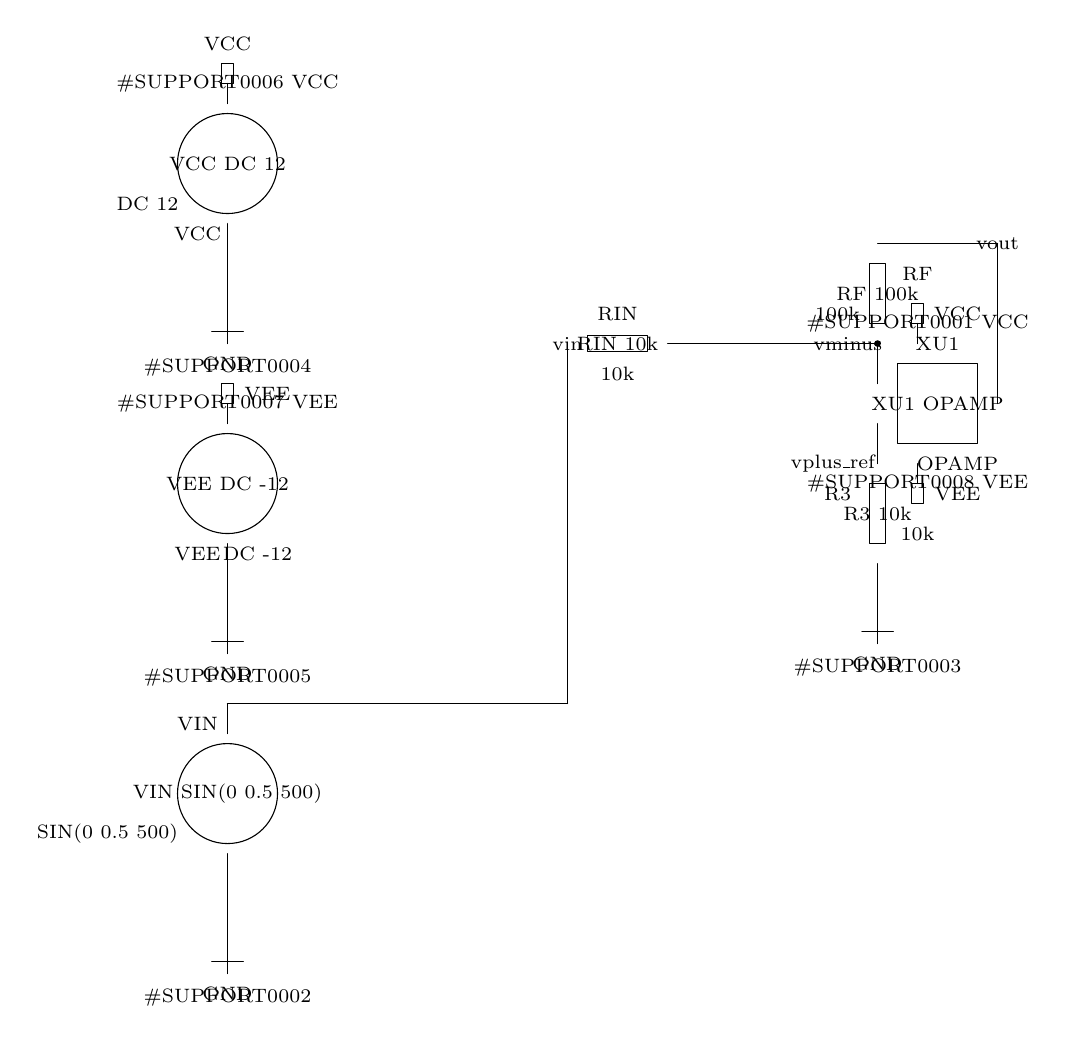
\begin{tikzpicture}[x=0.1cm,y=-0.1cm,line cap=round,line join=round]
  \draw (80.01,147.32) -- (80.01,160.02);
  \draw (162.56,110.49) -- (162.56,118.11);
  \draw (80.01,107.95) -- (80.01,119.38);
  \draw (80.01,67.31) -- (80.01,80.01);
  \draw (80.01,52.07) -- (80.01,49.53);
  \draw (167.64,82.55) -- (167.64,80.01);
  \draw (167.64,97.79) -- (167.64,100.33);
  \draw (80.01,92.71) -- (80.01,90.17);
  \draw (80.01,132.08) -- (80.01,128.27);
  \draw (80.01,128.27) -- (123.19,128.27);
  \draw (123.19,128.27) -- (123.19,82.55);
  \draw (162.56,87.63) -- (162.56,82.55);
  \draw (135.89,82.55) -- (162.56,82.55);
  \draw (177.80,90.17) -- (177.80,69.85);
  \draw (162.56,69.85) -- (177.80,69.85);
  \draw (162.56,92.71) -- (162.56,97.79);
  \fill (162.56,82.55) circle (1.2pt);
  \draw (80.01,59.69) circle (6.35);
  \node[font=\scriptsize,align=center] at (80.01,59.69) {VCC DC 12};
  \draw (165.10,85.09) rectangle (175.26,95.25);
  \node[font=\scriptsize,align=center] at (170.18,90.17) {XU1 OPAMP};
  \draw (161.54,72.39) rectangle (163.58,80.01);
  \node[font=\scriptsize,align=center] at (162.56,76.20) {RF 100k};
  \draw (125.73,81.53) rectangle (133.35,83.57);
  \node[font=\scriptsize,align=center] at (129.54,82.55) {RIN 10k};
  \draw (161.54,100.33) rectangle (163.58,107.95);
  \node[font=\scriptsize,align=center] at (162.56,104.14) {R3 10k};
  \draw (80.01,100.33) circle (6.35);
  \node[font=\scriptsize,align=center] at (80.01,100.33) {VEE DC -12};
  \draw (80.01,139.70) circle (6.35);
  \node[font=\scriptsize,align=center] at (80.01,139.70) {VIN SIN(0 0.5 500)};
  \draw (166.88,77.47) rectangle (168.40,80.01);
  \node[font=\scriptsize,align=center] at (167.64,80.01) {\#SUPPORT0001 VCC};
  \draw (80.01,160.02) -- (80.01,162.56);
  \draw (78.01,161.06) -- (82.01,161.06);
  \node[font=\scriptsize] at (80.01,165.56) {\#SUPPORT0002};
  \draw (162.56,118.11) -- (162.56,120.65);
  \draw (160.56,119.15) -- (164.56,119.15);
  \node[font=\scriptsize] at (162.56,123.65) {\#SUPPORT0003};
  \draw (80.01,80.01) -- (80.01,82.55);
  \draw (78.01,81.05) -- (82.01,81.05);
  \node[font=\scriptsize] at (80.01,85.55) {\#SUPPORT0004};
  \draw (80.01,119.38) -- (80.01,121.92);
  \draw (78.01,120.42) -- (82.01,120.42);
  \node[font=\scriptsize] at (80.01,124.92) {\#SUPPORT0005};
  \draw (79.25,46.99) rectangle (80.77,49.53);
  \node[font=\scriptsize,align=center] at (80.01,49.53) {\#SUPPORT0006 VCC};
  \draw (79.25,87.63) rectangle (80.77,90.17);
  \node[font=\scriptsize,align=center] at (80.01,90.17) {\#SUPPORT0007 VEE};
  \draw (166.88,100.33) rectangle (168.40,102.87);
  \node[font=\scriptsize,align=center] at (167.64,100.33) {\#SUPPORT0008 VEE};
  \node[font=\scriptsize] at (76.20,68.58) {VCC};
  \node[font=\scriptsize] at (69.85,64.77) {DC 12};
  \node[font=\scriptsize] at (170.18,82.55) {XU1};
  \node[font=\scriptsize] at (172.72,97.79) {OPAMP};
  \node[font=\scriptsize] at (167.64,73.66) {RF};
  \node[font=\scriptsize] at (157.48,78.74) {100k};
  \node[font=\scriptsize] at (129.54,78.74) {RIN};
  \node[font=\scriptsize] at (129.54,86.36) {10k};
  \node[font=\scriptsize] at (157.48,101.60) {R3};
  \node[font=\scriptsize] at (167.64,106.68) {10k};
  \node[font=\scriptsize] at (76.20,109.22) {VEE};
  \node[font=\scriptsize] at (83.82,109.22) {DC -12};
  \node[font=\scriptsize] at (76.20,130.81) {VIN};
  \node[font=\scriptsize] at (64.77,144.78) {SIN(0 0.5 500)};
  \node[font=\scriptsize] at (172.72,78.74) {VCC};
  \node[font=\scriptsize] at (80.01,165.10) {GND};
  \node[font=\scriptsize] at (162.56,123.19) {GND};
  \node[font=\scriptsize] at (80.01,85.09) {GND};
  \node[font=\scriptsize] at (80.01,124.46) {GND};
  \node[font=\scriptsize] at (80.01,44.45) {VCC};
  \node[font=\scriptsize] at (85.09,88.90) {VEE};
  \node[font=\scriptsize] at (172.72,101.60) {VEE};
  \node[font=\scriptsize] at (156.89,97.79) {vplus\_ref};
  \node[font=\scriptsize] at (158.78,82.55) {vminus};
  \node[font=\scriptsize] at (123.19,82.55) {vin};
  \node[font=\scriptsize] at (177.80,69.85) {vout};
\end{tikzpicture}
\section{Reference Summary}
\begin{longtable}{p{0.16\linewidth}p{0.18\linewidth}p{0.30\linewidth}p{0.22\linewidth}}
\textbf{Ref} & \textbf{Kind} & \textbf{Value / Model} & \textbf{Nodes}\\
\hline
VCC & V & DC 12 & vcc, 0\\
VEE & V & DC -12 & vee, 0\\
VIN & V & SIN(0 0.5 500) & vin, 0\\
RIN & R & 10k & vin, vminus\\
RF & R & 100k & vout, vminus\\
R3 & R & 10k & vplus\_ref, 0\\
XU1 & X & OPAMP & vplus\_ref, vminus, vout, vcc, vee\\
\end{longtable}

\paragraph{Analyses}
\begin{itemize}
  \item \texttt{tran 0.1ms 10ms}
\end{itemize}
\section{Design Notes}
\subsection*{Overview}
This generated example captures the opamp inverting circuit using voltage sources, voltage sources, voltage sources, and related support parts.

\subsection*{Operating Notes}
\begin{itemize}
  \item Primary simulation commands: tran 0.1ms 10ms.
  \item Component count: 7 active entries in the shared CircuitSpec.
  \item Named nets to review during edits: vcc, vee, vin, vminus, vout, vplus\_ref.
  \item Custom device models are embedded for 5 statements.
\end{itemize}
\subsection*{Design Notes To Edit}
\begin{itemize}
  \item Replace these starter notes with intended operating limits, tuning guidance, and simulation expectations.
  \item Record any KiCad-specific layout conventions that should stay aligned with the generated schematic.
  \item Add usage notes for the ngspice analyses that matter for this example.
\end{itemize}
\end{document}
